% !TeX root = ../main.tex
% -*- coding: utf-8 -*-
% !TeX root = ../main.tex
% -*- coding: utf-8 -*-

\chapter{绪论}
\label{chpt:introduction}
本章首先阐述本文的选题背景和意义,然后介绍软件重构机会推荐的相关研宄内容,接着阐述论文的主要工作和创
新点,最后介绍论文结构安排。

\section{研究背景与意义}

\subsection{软件质量与软件重构}
软件质量包括软件扩展性、模块性、可重构性、复杂性、可维护性、效率等方面~\cite{Boehm}。在软件演化过程
中,随着软件的不断改进以适应新的需求,其规模越来越大,代码结构也随之变得更复杂,导致了软件质量的降
低。为了提高软件质量,软件维护人员花费了大量的时间来理解和维护软件~\cite{Bansiya2002}。在软件生命周
期中,软件维护和演化的成本占总成本的80\%以上~\cite{guimaraes1983managing, coleman1994using}。

软件重构是提高软件质量,降低软件维护成本的重要手段之一。重构这个术语最早是由William
Opdyke~\cite{opdyke1992refactoring}在其博士论文中提出的。软件重构技术旨在在不改变软件整体功能的前提
下,改进软件的设计结构,使得新的设计结构提高代码的可维护性,从而提高软件的质量
~\cite{fowler1999refactoring}。因此,软件重构通常只改变软件的外观,比如在传统的结构化设计上以改进其
结构。软件重构不涉及修改软件的语义和功能,而是通过更好的观察软件系统,从而提出对软件系统设计各方面的
改进~\cite{chikofsky1990reverse}。软件重构通常是面向对象的软件重构,因此其主要通过改变类的层次结构和
其数据方法来重新设计面向对象的软件系统,以便提高软件质量。


\begin{figure}
  \centering
  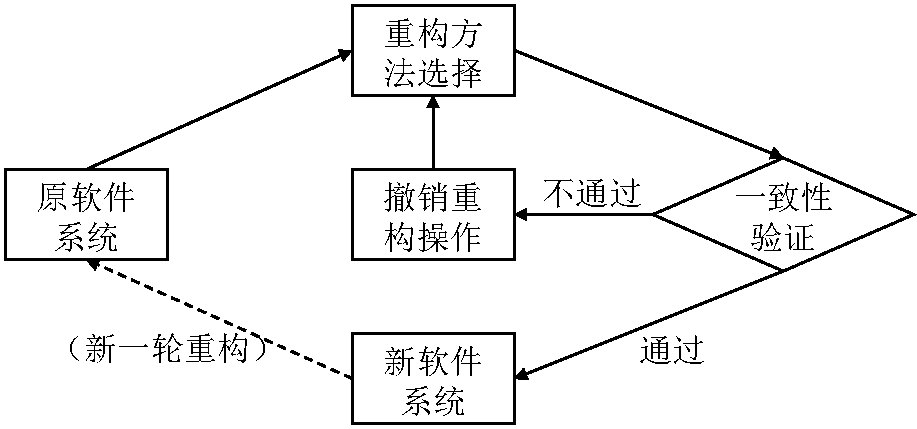
\includegraphics[height=45mm, width=90mm]{refactory.pdf}  
  \caption{\label{fig:refactory}软件重构一般过程}
\end{figure}

软件重构的一般是通过迭代转换的方式对软件系统进行转换。图~\ref{fig:refactory}描述了这样的转换过程。针
对原软件系统,每一轮迭代是对软件的一次小规模转换,针对特定代码选择某种重构方法,在实施软件重构操作后
测试其正确性,即测试软件的语义和功能是否与原来的保持一致。若测试通过,则本轮重构完成,软件维护人员可
在新的软件系统上进行新一轮重构。在任何时间一旦测试不通过,则最后一次程序转换撤销,需要重新选择重构方
法,换一种方式进行重构。通过很多轮这样的小规模程序转换,软件重构的过程和细节可以完全被软件维护人员所
掌控,并达到其所预想的效果。这样的迭代过程要求测试过程十分迅速,否则软件维护人员将不得不花费大量的时
间等待测试完成。因此,很多极限编程和其它敏捷软件开发的使用者将这种迭代过程作为软件开发周期的一个重要
组成部分。除此以外,为了减少一致性验证所带来的测试时间成本,部分学者提出使用先置性条件过滤,使得满足
条件的软件重构能保持语义和功能的一致性,从而减少不必要的测试成本。

研究者们提出了很多面向软件重构的技术和工具,主要可以分为两类:手动和自动化的方法。第一类方法主要通过
开发工具来为特定类型的手动重构操作提供技术支持~\cite{fowler1999refactoring, murphy2012we}。很多编辑
器和集成开发环境(IDE)如Eclipse等集成了这类重构支持工具,其作用仅仅是替软件维护人员执行指定的重构操
作。这类方法依赖于软件维护人员来识别软件重构机会和选择软件重构操作。因此,手动重构的过程较为复杂和乏
味,软件维护人员需要花费大量的时间和精力指定需要被执行的软件重构操作。第二类方法通过自动推荐可以被软
件维护人员直接采用的重构序列来提高软件质量\cite{harman2007pareto, kessentini2011design,
ouni2013maintainability, Silva2014}。这种序列可以是一个完整的重构方案,即软件维护人员必须接受完整的
解决方案;也可以是针对特定重构类型的推荐序列,维护人员可以通过逐步交互的方法来完全控制他们所要应用的
重构,通过有针对性的修复来提高软件质量。

大量的实践和研究表明,软件重构的作用主要有以下两种:(1)提高软件可维护性。当软件容易被理解时,软
件中的错误更容易被发现和修复~\cite{martin2009clean}。软件重构通过改进软件设计、重命名等方式,使得软
件设计更简单灵活、层次结构更清晰、代码更易被理解,从而减少代码维护的成本。(2)提高软件可扩展性。在
软件生命周期中,新的需求被不断添加,使得代码的复杂度越来越高,代码结构逐渐偏离原来的设计,从而导致了
扩展软件的难度越来越大。软件重构增加了程序设计的灵活性,通过改进软件设计,使得软件具备高凝聚、低耦合
和复杂度低等特点,将复杂代码变简单,从而提高代码的可扩展性。

\subsection{代码坏味与软件重构操作}
软件重构的时机通常与软件系统质量有关。软件质量下降时,软件系统发出需要重构的信号。最常见的情况是当软
件维护人员修补错误或添加新功能时,首先要需要做的就是理解代码。当代码可读性强,容易被理解时,修复软件
错误和添加新功能的效率更高。相反,当代码复杂度高、不容易被理解时,代码的质量下降,可维护性也随之降
低,此时通常需要对软件进行重构。重构软件可以加速当前和未来对代码的理解,从而提高软件维护效率。

代码坏味是软件系统中出现``坏代码''的信号,通常被研究者认为软件系统需要进行重构的信号。Fowler等人提出
了22种软件结构作为代码坏味的表现,并认为这些代码坏味可以帮助软件维护人员决定软件是否需要被重构
~\cite{fowler1999refactoring}。同时,Fowler等人提出了72代码重构操作,在保持程序外在行为的一致性的同
时,改进程序内部的设计结构~\cite{fowler1999refactoring}。在表~\ref{fig:badsmell}中我们列举了其中十种
经典的代码坏味,以及可能解决这些代码坏味的软件重构操作。

\begin{center}
\tablecaption{十种经典代码坏味}\label{fig:badsmell}
\begin{tabular}{|l|l|l|l|}
\hline
序号 & 代码坏味 & 软件重构操作 & 重构目标\\ \hline
1 & 代码重复 & 函数提炼、函数上移、类提炼 & 提取公共代码\\ \hline
2 & 函数过长 & 函数提炼 & 拆分函数\\ \hline
3 & 类过大 & 类提炼 & 拆分类\\ \hline
4 & 参数过多 & 引入参数对象、函数替代参数 & 减少参数\\ \hline
5 & 发散式变化& 类提炼 & 将全部变化提取到新类\\ \hline
6 & 霰弹式改动& 函数移动、类内联 & 将全部修改合并为同类\\ \hline
7 & 依恋情节& 函数提炼、函数移动 & 移动依恋代码\\ \hline
8 & 数据泥团& 类提炼、引入参数对象 & 简化数据\\ \hline
9 & 基本类型偏执& 对象替换数据 & 简化类型 \\ \hline
10 & Switch语句 & 函数提炼、函数移动 & 减少Switch语句\\ \hline
\end{tabular}
\end{center}

值得注意的是,每一种代码坏味可以被一种或多种软件重构操作所解决。如表~\ref{fig:badsmell}中的代码重
复,在很多情况下可以通过函数提炼(Extract Method)提取重复的代码结构作为一个新的函数被调用;当重复代
码出现在两个兄弟子类时,可以分别在这两个子类中进行函数提炼,然后将该函数上移(Pull Up Method)到这两
个子类的父类中;当重复代码出现在两个不相干的类中时,可以将重复代码提取为一个新类(Extract Class),
在原来的两个类中调用这个新类。因此我们可以看出,即使针对同一代码坏味,在不同的情况下软件维护人员需要
选择不同的重构操作,甚至是一系列重构操作的叠加。

代码坏味不完全是相互独立的,有一些代码坏味是相关联的,因此可以被相同的软件重构操作所解决。例如代码重
复可能会导致函数过长或者类过大,此时如果使用函数提炼或类提炼,既解决了代码重复的问题,同时也解决了函
数过长或者类过大的问题。同样,依恋情节通常发生在某个函数对某个类的兴趣远高于其所在的类,此时会导致该
函数频繁的访问该类,可能导致函数过长、类过大、参数过多以及发散式变化(容易受到该类的影响)等代码坏
味。通过将部分依恋代码提炼成新的函数,并移动到其频繁访问的类(Move Method),可以让大部分问题得到改
善。

有一些代码坏味是互斥的,因此它们所对应的软件重构操作也是互为逆向操作。如表~\ref{fig:badsmell}中的类
过大和霰弹式改动是两个互斥的代码坏味。当我们用类提炼将大类拆分成多个小类时,虽然每个类的规模变小,但
容易引发霰弹式改动的问题,即原来在同一个大类中的多个小类由于彼此依赖,导致当改动其中一个小问题时,引
发一系列发散的改动,造成软件维护的不便;反之,当我们用类内联(Inline Class)将某个修改所涉及到的修改
都集合到同一个大类中时,虽然解决了霰弹式改动的代码坏味,但此时容易引起类过大的问题。这样逆向的软件重
构操作还有函数提炼和函数内联(Inline Method)、函数上移和函数下移(Pull Down Method)等。因此,如何
针对软件系统选取合适的软件重构操作是软件维护人员需要解决的问题。

虽然代码坏味是软件重构的重要信号,但是软件重构的动机却不完全是为了解决代码坏味。Silva等人
~\cite{Silva2016}调查研究了软件开发人员进行软件重构的动机。调查发现,软件重构主要发生在需求发生改变
的时候,如增加新特性或是修复软件错误时,因此软件重构的动机通常与提高软件的易读性、可重用性、易测性等
相关,而不仅仅是针对特定代码坏味的修复。以最常用的软件重构操作--函数提炼为例,调查显示,软件维护人员
进行函数提炼重构的原因较为复杂,包括代码重用、函数分解、加速扩展、重命名内部函数等11种主要原因。其
中,只有函数分解与代码坏味有关,其通常被认为是解决代码坏味``函数过长''的方法。由于人工识别软件重构机
会并选择软件重构操作的成本较高,且软件重构的动机具有复杂性和多样性,研究者们提出了很多软件重构推荐技
术来解决该问题,关于软件重构推荐的研究引起了广泛关注。

\section{软件重构技术相关研究现状}
软件重构的一般过程是选定待重构代码,然后选择软件重构操作,在进行重构后对软件的一致性进行检测,确保该
软件重构操作没有改变软件原有的语义和功能。由于软件重构原因和过程的复杂性,导致软件维护人员需要根据自
己对软件系统的理解,不断做出决策,耗费大量的时间和精力成本。尤其是当重构操作涉及到不止一个文件和代码
包时~\cite{liu2013monitor},因此,自动软件重构技术越来越得到研究者们的关注。目前,大多数集成开发环
境,如Eclipse和IntelliJ IDEA等,提供了软件重构的支持工具作为插件。 以Eclipse为例,当开发人员需要重构
时,首先选择待重构代码,然后选定软件重构类型以及必要的输入(如函数重命名操作中的新函数名),Elipse可
以替代软件维护人员完成剩下的工作。这样的工具为自动和半自动化软件重构提供了基础,是软件重构被广泛应用
的重要因素~\cite{griswold1993automated,tip2003refactoring,mens2005formalizing}。本节首先介绍软件重构
操作的自动检测技术,然后介绍软件重构推荐的相关技术,包括软件重构机会的识别和推荐,以及软件重构顺序推
荐,最后介绍软件重构的一致性相关研究。

\subsection{软件重构检测}

软件重构检测通过检测相同软件系统不同版本之间发生的软件重构操作,帮助软件维护人员熟悉代码改变的意图,
更好地了解软件的演化过程。Robbes等人~\cite{robbes2008spyware}开发了一个工具集Spyware来监视集成开发环
境。该工具将软件开发人员对代码的修改表示为基于语义的修改序列,并将这些重要的修改存储起来,开发者可以
通过观察和重放这些修改来观测到软件重构的发生。

大多数研究者主要通过比较两个软件版本中代码的相似度来检测软件重构。Demeyer等人
~\cite{demeyer2000finding}首次提出通过比较相同软件系统的不同版本来检测软件重构的方法,该方法通过比较
软件度量,如代码行数(LOC)和函数调用个数等,检测是否存在软件重构。Malpohl等人
~\cite{malpohl2003renaming}通过使用diff命令来比较两个函数的相似度,从而推测出函数重命名的重构操作。
Antoniol等人~\cite{antoniol2004automatic}提出了基于向量空间的信息检索方法检测代码重构。Xing等人
~\cite{xing2005umldiff}基于命名和结构相似度,自上之下比较了包、类、借口等程序元素。同样基于相似度原
理,部分研究者将克隆检测器应用于软件重构检测中,将不同版本的函数相对应,从而检测出函数提炼和函数移动
等软件重构操作~\cite{van2003reconstruction,kim2005functions}。Weißgerber等人
~\cite{weissgerber2006identifying}提出将软件仓库通过预处理存储进关系型数据库中,然后将每次提交的代码
修改作为事务创建,从中分析出增加、修改或删除的类、字段和函数,从而得到可能的软件重构操作,最后使用克
隆检测将这些操作排序。

由于软件重构的本质是保持软件的语义不变,改变其内部结构,因此有研究者提出使用基于语义分析的方法检测软
件重构。Dig等人~\cite{dig2006automated}开发了基于Eclipse的插件,其首先通过语义分析函数调用、类型使
用、实例化等关系,然后使用一种迭代的方法自顶而下的检测重构。Fluri等人~\cite{fluri2007change}比较了两
个版本的抽象语法树,计算了基于抽象语法树的修改操作,并将其映射到抽象语法树级别的代码修改上。这种方法
的优点在于识别了语法树级别的原子改变,但是由于其停留在原子改变,而未将多处改变抽象化分析,导致其很难
检测出更抽象级别的软件重构。

由于基于相似度比较的软件重构检测方法,其侧重点在于不同版本的软件系统的比较,导致其所能检测出的软件重
构的类型有限,大多为函数移动、函数重命名等简单的重构类型;而复杂重构类型往往涉及多处修改,因此很难被
基于相似度比较的方法检测到。Taneja等人~\cite{taneja2007automated}开发了一种工具RefacLib,通过句法分
析来检测代码库的不同版本之间可能存在的软件重构操作。Kim等人~\cite{kim2007automatic}提出了一种基于规
则的识别代码修改的方法,发现并总结了代码改变的逻辑规则,通过自动匹配不同软件系统的函数并根据该逻辑规
则检测软件重构。Xing等人~\cite{xing2006refactoring}将32种特定类型的软件重构表示成查询语句,提出了基
于代码改变的查询方法,将不同软件版本在软件设计的改变提取到数据库中,查询满足软件重构规则的重构操作实
例。Prete等人~\cite{prete2010template}提出了基于逻辑的方法来检测软件重构,根据模板逻辑规则将每个重构
类型表示出来,并使用逻辑编程引擎来推测重构实例。他们开发了工具Ref-Finder,从代码结构上分析了63种软件
重构类型所对应的重构前后的改变。

\subsection{软件重构机会推荐}
虽然半自动的软件重构过程可以省去不必要的人工操作和验证,但其仍然依赖于程序员对软件系统的理解来做出一
系列适合当前软件系统的决策。为了提高软件重构效率,已经有很多工作致力于软件重构机会的识别和推荐。关于
软件重构机会推荐的工作通常包括两个方面,分别是软件重构机会的识别和软件重构操作推荐。这两个方面分别对
应着软件重构的两个关键步骤:(1)识别选定代码是否存在软件重构机会(2)为选定代码推荐合适的软件重构操
作。通常情况下,只有识别了软件重构机会,才有可能对软件进行重构。而人工识别软件重构机会往往要求软件维
护人员对软件系统的设计和实现有全局的了解,因此对软件维护人员的经验和能力要求较高,尤其是在不用程序分
析工具的情况下,了解软件系统的设计并识别软件重构机会是一个复杂而耗时的过程。值得注意的是,部分研究将
这两个步骤融合在一起,在识别软件重构机会的同时推荐重构操作。例如,当我们对代码进行克隆检测
~\cite{kamiya2002ccfinder}的同时,如果我们检测到了克隆代码,往往使用函数提炼或类提炼等重构将公共代码
提取出来,以便复用。根据主要方法的不同,我们可以将关于软件重构机会推荐的研究分为六类
~\cite{al2015identifying}。

 

\subsubsection{基于软件质量度量的重构机会推荐}
\subsubsection{基于前置条件的重构机会推荐}
\subsubsection{基于聚类的重构机会推荐}
\subsubsection{基于图的重构机会推荐}
\subsubsection{基于代码切片的重构机会推荐}
\subsubsection{基于动态分析的重构机会推荐}

\subsection{软件重构顺序}
\subsection{软件重构一致性验证}
\subsection{软件重构工具}

\section{本文的主要工作与创新点}

\section{论文的结构安排}

本模板参照南开大学学位论文写作规范编写,
仅仅提供了论文的基本格式,包括章节标题和正文字体、字号等等的设置。



您自愿使用这个模板。
提供本模板的目的是为了给您的论文写作带来方便,然而,
作者不保证这个模板完全符合学校的要求,也不对由此产生的任何后果负责。
如果您不同意这些条款,请不要使用这个模板。


\section{常用内容}

\begin{itemize}
	\item 参考文献的录入请参考\ref{sec:relatedwork:ref};
	\item 图片插入参考\ref{sec:relatedwork:table};
	\item 分数和公式参考\ref{sec:relatedwork:equation};
	\item Latex绘图工具参考\ref{sec:method:tikz};
	\item 代码块参考\ref{sec:method:code};
\end{itemize}